% !TEX encoding = UTF-8 Unicode.

% Based on https://github.com/Miracle0565/BUCT-Beamer-Theme

\documentclass[
10pt,
aspectratio=43,
]{beamer}
\setbeamercovered{transparent=10}
\usetheme[
%  showheader,
%  red,
  purple,
%  gray,
%  graytitle,
  colorblocks,
%  noframetitlerule,
]{Verona}

\usepackage[T1]{fontenc}
\usepackage{tikz}
\usepackage[utf8]{inputenc}
\usepackage{lipsum}
%%%%%%%%%%%%%%%%%%%%%%%%%%%%%%%
% Mac上使用如下命令声明隶书字体,windows也有相关方式,大家可自行修改
\providecommand{\lishu}{\CJKfamily{zhli}}
%%%%%%%%%%%%%%%%%%%%%%%%%%%%%%%
\usepackage{tikz}
\usetikzlibrary{fadings}
%
%\setbeamertemplate{sections/subsections in toc}[ball]
\usepackage{xeCJK}
\usepackage{listings}
\usepackage{caption}
\usepackage{subfigure}
\usefonttheme{professionalfonts}
\def\mathfamilydefault{\rmdefault}
\usepackage{amsmath}
\usepackage{multirow}
\usepackage{booktabs}
\usepackage{bm}
\setbeamertemplate{section in toc}{\hspace*{1em}\inserttocsectionnumber.~\inserttocsection\par}
\setbeamertemplate{subsection in toc}{\hspace*{2em}\inserttocsectionnumber.\inserttocsubsectionnumber.~\inserttocsubsection\par}
\setbeamerfont{subsection in toc}{size=\small}
\AtBeginSection[]{%
	\begin{frame}%
		\frametitle{Outline}%
		\textbf{\tableofcontents[currentsection]} %
	\end{frame}%
}

\AtBeginSubsection[]{%
	\begin{frame}%
		\frametitle{Outline}%
		\textbf{\tableofcontents[currentsection, currentsubsection]} %
	\end{frame}%
}

\title{高等数学C}
%\subtitle{A Simple while elegant template}
\author[P.Yu]{余沛}
\mail{peiy\_gzgs@qq.com}
\institute[Guangzhou College of Technology and Business]{Guangzhou College of Technology and Business \\
  广州工商学院}
\date{\today}
\titlegraphic[width=4cm]{logo.png}{}




%%%%%%%%%%%%%%%%%%%%%%%%%%%%%%%%
% ----------- 标题页 ------------
%%%%%%%%%%%%%%%%%%%%%%%%%%%%%%%%



\begin{document}

\maketitle

%%% define code
\defverbatim[colored]\lstI{
	\begin{lstlisting}[language=C++,basicstyle=\ttfamily,keywordstyle=\color{red}]
	int main() {
	// Define variables at the beginning
	// of the block, as in C:
	CStash intStash, stringStash;
	int i;
	char* cp;
	ifstream in;
	string line;
	[...]
	\end{lstlisting}
}
%%%%%%%%%%%%%%%%%%%%%%%%%%%%%%%%
% ----------- FRAME ------------
%%%%%%%%%%%%%%%%%%%%%%%%%%%%%%%%

\section{变量变化问题}
\subsection{速度问题-I} % 匀速运动的情形
\begin{frame}{变量变化问题}{速度问题-I: 匀速运动的情形}
	考虑某物体 $A$ 以速度 $v$ 运动的情形, 记 $t$ 为物体运动的经过时间长度, $s$ 为物体在 $t$ 时刻运动的路程, 我们有
	\[
		s(t) = v\cdot t.
	\]
	对于时刻 $t_1$, $t_2$ 来说, 我们有
	\[
		s(t_2) = v\cdot t_2 = v\cdot t_1 + v\cdot (t_2-t_1) = s(t_1) + v \cdot (t_2-t_1).
	\]
	也就是说
	\[
		s(t_2) - s(t_1) = v \cdot (t_2-t_1), \quad v=\frac{s(t_2)-s(t_1)}{t_2-t_1}.
	\]
\end{frame}

\subsection{速度问题-II} % 匀加速运动的情形

\begin{frame}{变量变化问题}{速度问题-II: 匀加速运动的情形}
	考虑某物体 $A$ 以初速度 $v_0$, 加速度 $a$ 运动的情形, 记 $t$ 为物体运动的经过时间长度, $v(t)$ 为物体在$t$时刻的速度, $s(t)$ 为物体在 $t$ 时刻运动的路程, 我们有
	\[
		v(t) = v_0+a\cdot t.
	\]
	对于时刻 $t_1$, $t_2$ 来说, 我们有
	\[
		v(t_2) = a\cdot t_2 = a\cdot t_1 + a\cdot (t_2-t_1) = v(t_1) + a \cdot (t_2-t_1).
	\]
	也就是说
	\[
		v(t_2) - v(t_1) = a \cdot (t_2-t_1), \quad a=\frac{v(t_2)-v(t_1)}{t_2-t_1}.
	\]
\end{frame}

\begin{frame}{变量变化问题}{速度问题-II: 匀加速运动的情形}
	在前序知识中, 我们知道下式子以及相关的变形,
	\[
		s(t) = v_0\cdot t+ \frac{1}{2}a\cdot t^2
	\]
	那么有
	\begin{align*}
		s(t_2) - s(t_1) & = v_0\cdot (t_2-t_1)+ \frac{1}{2}a\cdot (t_2^2-t_1^2)            \\
		                & =v_0\cdot(t_2-t_1) + a\cdot(t_2-t_1) \cdot \frac{1}{2}(t_2+t_1), 
	\end{align*}
	即
	\begin{align*}
		\frac{s(t_2) - s(t_1)}{t_2-t_1} = v_0 + a\cdot \frac{1}{2}(t_2+t_1). 
	\end{align*}
	对比匀速运动的速度定义, 我们可以看到, $t_1\sim t_2$ 期间的平均速度
	\begin{equation*}
		\tilde{v}=\frac{s(t_2) - s(t_1)}{t_2-t_1} = v_0 + a\cdot \frac{1}{2}(t_2+t_1).
	\end{equation*}
	我们考虑速度 $t_2$, $t_1$ 足够接近的情况, $\lim_{(t_2-t_1)\to 0}\tilde{v}=v_0+a\cdot t_1$, 一致?
\end{frame}

\subsection{速度问题-III} % 一般加速运动的情形
\begin{frame}{变量变化问题}{速度问题-II: 匀加速运动的情形}
	\begin{exampleblock}{高超声速飞行器速度问题 \color{blue}(\small{\it 郭建国等, {现代防御技术}, 49(6) 2021.12.)}}
		平飞高超声速飞行器的加速度 $a$ 的简化计算模型为: 
		\begin{align*}
			m\cdot a(t)= \frac{1}{2}\rho(s) v(t)^2 S C_T, 
		\end{align*}
		其中, $m$ 是飞行器质量, $v(t)$ 是飞行器速度, $\rho(s)$ 是大气密度, $S$ 是飞行器截面积参考参数, $C_T$ 是油门控制值. 这种问题, 只给出$\rho(s)$, $S$, $C_T$ 和初速度, 如何计算路程和速度?	
	\end{exampleblock}
	思路: 极限求 $v(t)$, 逐步求解. 对于 $t_2$, $t_1$ 足够接近的时候,
	\[
		v(t_2)\approx v(t_1)+a\left(\frac{t_2+t_1}{2}\right)(t_2-t_1).
	\]
	即
	\[
		\frac{v(t_2)-v(t_1)}{t_2-t_1}\approx a\left(\frac{t_2+t_1}{2}\right)(t_2-t_1).
	\]
	因而, 我们会考虑相关的极限问题.
\end{frame}


\subsection{函数的切线问题-I} % 二次函数的切线问题

\begin{frame}{变量变化问题}{切线问题-II: 二次函数的情形}
	考虑二次函数
		
	\[
		f(x) = a\cdot x^2 + b\cdot x +c.	
	\]
	先序教育中, 给出了一些特殊函数的求导方法, 
	\[
		k = f'(x0) = 2  a \cdot x0 + b
	\]
	也定义了在某点上的切线方程,
	\[
		y = k \cdot x + (f(x0) - k \cdot x0),
	\]
	可以看到切线和导数之间具有某种关系.
\end{frame}


\subsection{函数的切线问题-I} % 一般函数的切线问题

\begin{frame}{变量变化问题}{切线问题-II: 一般函数的情形}
	考虑函数 $f(x)$ 在点 $(x_0,f(x_0))$ 的切线问题,
	考虑 $x_1<x_0<x_2$, 两点 $(x_1,f(x_1))$, $(x_2,f(x_2))$ 两点的割线斜率是
	\[
		k=\frac{f(x_2)-f(x_1)}{x_2-x_1},
	\]
	相关的割线方程是
	\[
		y-f(x_1)=k\cdot(x-x_1).
	\]
	
	\begin{center}
		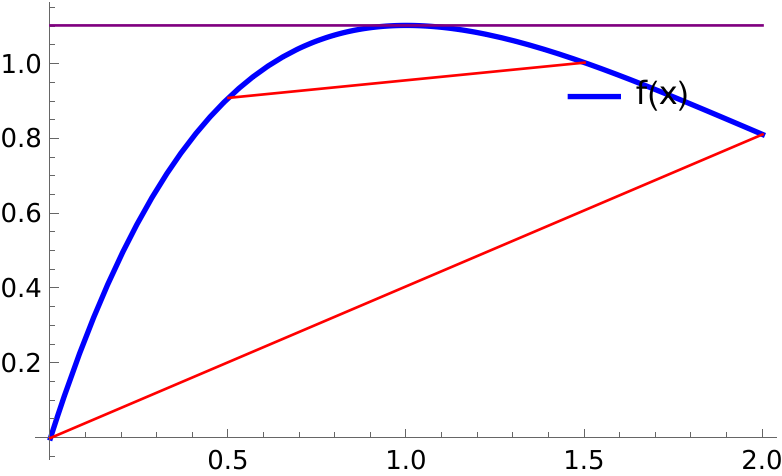
\includegraphics[scale=0.5]{tangent secant.png}	
	\end{center}
	同样,用割线逼近切线, $x_1,x_2\to x_0$, $f(x)$ 的割线会慢慢逼近于切线
\end{frame}

\section{导数}
\subsection{导数的定义}
\begin{frame}{导数的定义}
	\begin{block}{定义:函数导数}
		设 $f$, $\delta>0$ $(x_0-\delta,x_0+\delta)$, (或 $(x_0-\delta,x_0], [x_0,x_0+\delta)$) 上有定义, 对于 $0<\Delta x<\delta$, 如果极限 
		\begin{equation*}
			\begin{array}[c]{c}
				\displaystyle\lim_{\Delta x\to 0 } \frac{f(x_0+\Delta x)-f(x_0)}{\Delta x},\bigskip                                                                          \\
				\displaystyle\left(\text{或}\,\,\lim_{\Delta x\to0}\frac{f(x)-f(x-\Delta x)}{\Delta x}, \,\, \lim_{\Delta x\to0}\frac{f(x+\Delta x)-f(x)}{\Delta x} \right) 
			\end{array}
		\end{equation*}
		存在, 则称 $f$ 在 $x_0$ 处可导 (或左导数存在, 右导数存在), 则称该极限值为 $f$ 在 $x_0$ 处的导数或微商 (或 左导数, 右导数), 记为 $f'(x_0)$ (或 $f'_-(x_0)$, $f'_+(x_0)$).
	\end{block}
	\pause
	若左右导数都存在且相等, 那么导数存在, 并与前两者的值相等.
\end{frame}


\begin{frame}{求导方法}
	\begin{block}{求导流程}
		\begin{enumerate}
			\pause\item 	给出 $\Delta x$; 算出 $\Delta y$; 求增量
			\pause\item  	求增量比 $\frac{\Delta y}{\Delta x}$; 求差商
			\pause\item  	求极限.
		\end{enumerate}		
	\end{block}
\end{frame}


\begin{frame}{一些例子}
	\begin{block}{例子}
		\begin{enumerate}
			\item $f(x)=C$, \pause $f'(x) =0$;\pause
			\item $f(x)=x^n, (n\in\mathbb{N}^+)$, \pause $f'(x) = n x^{n-1}$;\pause
			\item $f(x)=\sin(x)$, \pause $f'(x)=\cos(x)$; \,\,\pause $g(x)=\cos(x)$, \pause $g'(x)=\sin(x)$;\pause 
			\item $f(x)=\log_a  x$,\pause $f'(x)=\log a \cdot \displaystyle\frac{1}{x}$
		\end{enumerate}		
	\end{block}
\end{frame}

\subsection{导数的四则运算法则}
\begin{frame}{函数和差的导数}
	\begin{block}{函数和差的导数}
		设 $f(x)$, $g(x)$ 在 $x_0$ 处有导数, 那么有
		\[
			(f(x_0)\pm g(x_0))' = f'(x_0)\pm g'(x_0).
		\]
	\end{block}
	\pause
	Why?
	\pause
	\begin{align*}
		  & \frac{(f(x_0+\Delta x)\pm g(x_0+\Delta x))-(f(x_0)\pm g(x_0))}{\Delta x}                  \\
		= & \frac{f(x_0+\Delta x)-f(x_0)}{\Delta x}\pm \frac{( g(x_0+\Delta x))-( g(x_0))}{\Delta x}. 
	\end{align*}
\end{frame}

\begin{frame}{函数和差的导数}{导数计算题目}
	\begin{block}{题目}
		计算以下函数的导数:
		\begin{enumerate}
			\item $f(x) = 1 + x$,
			\item $g(x) = x + \sin(x)$,
			\item $h(x) = \cos(x) + \log(x)$,
		\end{enumerate}
	\end{block}
			
	\pause
			
	\begin{block}{答案}
		\begin{enumerate}
			\item $f'(x) = 1$,
			\item $g'(x) = 1 + \cos(x)$,
			\item $h'(x) = -\sin(x) + \displaystyle\frac{1}{x}$,
		\end{enumerate}
	\end{block}
\end{frame}

\begin{frame}{函数乘积的导数}
	\begin{block}{函数乘积的导数}
		设 $f(x)$, $g(x)$ 在 $x_0$ 处有导数, 那么有
		\[
			(f(x_0)\cdot g(x_0))' = f'(x_0)\cdot g(x_0) + f(x_0)\cdot g'(x_0).
		\]
	\end{block}
	\pause
	Why?
	\pause
	\begin{align*}
		  & f(x_0+\Delta x)g(x_0+\Delta x)-f(x_0) g(x_0))                                                 \\\bigskip
		= & \left(f(x_0+\Delta x)g(x_0+\Delta x)-f(x_0) g(x_0+\Delta x)\right)                            \\\smallskip
		  & + \left(f(x_0)g(x_0+\Delta x)-f(x_0) g(x_0)\right)                                            \\\bigskip
		= & \left(f(x_0+\Delta x)-f(x_0)\right)g(x_0+\Delta x)+f(x_0)\left(g(x_0+\Delta x)-g(x_0)\right). 
	\end{align*}
\end{frame}

\begin{frame}
	\frametitle{函数乘积的导数}{导数计算题目}
		
	\begin{exampleblock}{题目}
		计算以下函数的导数:
		\begin{enumerate}
			\item $f(x) = x \log(x)$,
			\item $g(x) = x \sin(x)$,
			\item $h(x) = \sin(x) \cos(x) \log(x)$,
		\end{enumerate}
	\end{exampleblock}
		
	\pause
		
	\begin{exampleblock}{答案}
		\begin{enumerate}
			\item $f'(x) = \log(x) + 1$,
			\item $g'(x) = \sin(x) + x \cos(x)$,
			\item $h'(x) = \cos^2(x) \log(x) - \sin^2(x) \log(x) + \displaystyle\frac{\sin(x)\cos(x)}{x}$,
		\end{enumerate}
	\end{exampleblock}
		
\end{frame}

\begin{frame}{函数商的导数}
	\begin{block}{函数乘积的导数}
		设 $f(x)$, $g(x)$ 在 $x_0$ 处有导数, 且 $g'(x_0)\neq 0$, 那么有
		\[
			\left(\frac{f(x_0)}{g(x_0)}\right)' = \frac{f'(x_0)g(x_0)-g'(x_0)f(x_0)}{(g'(x_0))^2}
		\]
	\end{block}
	Why?
	\begin{align*}
		  & \frac{f(x_0+\Delta x)}{g(x_0+\Delta x)}-\frac{f(x_0)}{g(x_0)}                                                \\\bigskip 
		= & \frac{f(x_0+\Delta x)g(x_0)-f(x_0)g(x_0+\Delta x)}{g(x_0+\Delta x)g(x_0)}                                    \\\bigskip
		= & \frac{f(x_0+\Delta x)g(x_0)-f(x_0)g(x_0)+f(x_0)g(x_0)-f(x_0)g(x_0+\Delta x)}{g(x_0+\Delta x)g}               \\\bigskip
		= & \frac{\left(f(x_0+\Delta x)-f(x_0)\right)g(x_0)-f(x_0)\left(g(x_0+\Delta x)-g(x_0)\right)}{g(x_0+\Delta x)g} 
	\end{align*}
\end{frame}

\begin{frame}{函数商的导数}
	\frametitle{函数商的导数}{导数计算题目}
		
	\begin{exampleblock}{题目}
		计算以下函数的导数:
		\begin{enumerate}
			\item $f(x) = \sec(x)$, 注: $\left(\sec(x)=\displaystyle\frac{1}{\cos(x)}\right),$
			\item $g(x) = \tan(x)$,
			\item $h(x) = \displaystyle\frac{\cos(x)}{\log(x)}$,
		\end{enumerate}
	\end{exampleblock}
		
	\pause
		
	\begin{exampleblock}{答案}
		\begin{enumerate}
			\item $f'(x) = \sec(x) \tan(x)$,
			\item $g'(x) = \sec^2(x)$,
			\item $h'(x) = \displaystyle\frac{-\sin(x)\log(x)-\displaystyle\frac{\cos(x)}{x}}{(\log(x))^2}$,
		\end{enumerate}
	\end{exampleblock}
		
\end{frame}

\begin{frame}
	\frametitle{反函数求导定理}
		
	\begin{theorem}[定理 4.3.4]
		若函数 $y=f(x)$ 在 $(a, b)$ 上连续、严格单调、可导并且 $f'(x) \neq 0$,记 $\alpha=\min(f(a+), f(b-))$,$\beta=\max(f(a+), f(b-))$,则它的反函数 $x=f^{-1}(y)$ 在 $(\alpha, \beta)$ 上可导,且有
		\[
			\left[f^{-1}(y)\right]' = \frac{1}{f'(x)}.
		\]
	\end{theorem}
	
\end{frame}
\begin{frame}
	\frametitle{反函数求导定理}
	\begin{proof}
		因为函数 $y=f(x)$ 在 $(a, b)$ 上连续且严格单调,由反函数连续定理,它的反函数 $x=f^{-1}(y)$ 在 $(\alpha, \beta)$ 上存在、连续,且严格单调。这时 $\Delta y=f(x+\Delta x)-f(x) \neq 0$ 等价于 $\Delta x=f^{-1}(y+\Delta y)-f^{-1}(y) \neq 0$,并且当 $\Delta y \rightarrow 0$ 时有 $\Delta x \rightarrow 0$。因此
		\[
			\begin{aligned}
				\left[f^{-1}(y)\right]' & = \lim_{\Delta y \rightarrow 0} \frac{f^{-1}(y+\Delta y)-f^{-1}(y)}{\Delta y} \\
				                        & = \lim_{\Delta x \rightarrow 0} \frac{\Delta x}{f(x+\Delta x)-f(x)}           \\
				                        & = \frac{1}{\lim_{\Delta x \rightarrow 0} \frac{f(x+\Delta x)-f(x)}{\Delta x}} \\
				                        & = \frac{1}{f'(x)}.                                                            
			\end{aligned}
		\]
	\end{proof}
\end{frame}

\begin{frame}
	\frametitle{导数计算题目}
			
	\begin{exampleblock}{题目}
		计算以下函数的导数:
		\begin{enumerate}
			\item $f(x) = e^x,$
			\item $g(x) = \arcsin(x),$
			\item $h(x) = \arccos(x).$
		\end{enumerate}
	\end{exampleblock}
			
	\pause
			
	\begin{exampleblock}{答案}
		\begin{enumerate}
			\item $f'(x) = e^x$, 令 $y=e^x$, 有 $x=\log y$ 和 $(e^x)'=\displaystyle\frac{1}{(\log y)'}=y=e^x,$
			\item $g'(x) = \displaystyle\frac{1}{\sqrt{1-x^2}},$ $(\arcsin(x))'=\displaystyle\frac{1}{(\sin (y))'}=\frac{1}{\cos(y)}=\frac{1}{\sqrt{1-(\sin(y))^2}}=\frac{1}{\sqrt{1-x^2}},$
			\item $h'(x) = -\displaystyle\frac{1}{\sqrt{1-x^2}},$ 类似的, $(\arcsin(x))'=\displaystyle\frac{1}{(\sin (y))'}=-\frac{1}{\sqrt{1-x^2}}.$
		\end{enumerate}
	\end{exampleblock}
\end{frame}
	

\subsection{复合函数的求导法则}
\begin{frame}{复合函数的求导法则}
	\begin{block}{函数乘积的导数}
		如果 $u=\varphi(x)$ 在 $x=x_0$ 点可导, 且 $y=f(u)$, $u=u_0=\varphi\left(x_0\right)$ 点也可导, 那么, 复合函数 $f(\varphi(x))$ 在 $x=x_0$ 点可导
		\[
			[f(\varphi(x))]_{x=x_0}^{\prime}=f^{\prime}\left(u_0\right) \varphi^{\prime}\left(x_0\right)
		\]
	\end{block}
	Why? \pause 考虑 $\Delta u = u(x_0+\Delta x) - u(x_0)$, \pause 由连续性, 有$\lim_{\Delta x\to0}\Delta u=0$ \pause
	\begin{align*}
		f\left(u_0+\Delta u\right)-f\left(u_0\right)=f^{\prime}\left(u_0\right) \Delta u+\alpha(\Delta u) \Delta u 
	\end{align*}
	其中 $\lim_{\Delta x\to0}\alpha(\Delta u)=0$. \pause Why? \pause 
	\begin{align*}
		\lim _{\Delta x \rightarrow 0} \frac{f\left(g\left(x_0+\Delta x\right)\right)-f\left(g\left(x_0\right)\right)}{\Delta x}= & f^{\prime}\left(u_0\right) \lim _{\Delta x \rightarrow 0} \frac{\Delta u}{\Delta x}+\lim _{\Delta x \rightarrow 0} \alpha \lim _{\Delta x \rightarrow 0} \frac{\Delta u}{\Delta x} \\
		=                                                                                                                         & f^{\prime}\left(u_0\right)f^{\prime}\left(x_0\right).                                                                                                                              
	\end{align*}
\end{frame}


\begin{frame}
	\frametitle{导数计算题目}
	
	\begin{exampleblock}{题目}
		计算以下函数的导数:
		\begin{enumerate}
			\item $f(x) = x^a,$ Hint: $(log(f(x)))'=f'(x)(f(x))^{-1}$,
			\item $g(t) = A \sin(3t+2),$
			\item $h(x) = e^{\sqrt{1+\cos(x)}},$
			\item $k(x) = \arcsin(e^{-x^2}),$
		\end{enumerate}
	\end{exampleblock}
	
	\pause
	
	\begin{exampleblock}{答案}
		\begin{enumerate}
			\item $f'(x) = ax^{a-1},$
			\item $g'(t) = 3A \cos(3t+2),$
			\item $h'(x) = \displaystyle\frac{\sin(x)}{2\sqrt{1+\cos(x)}}e^{\sqrt{1+\cos(x)}},$
			\item $k'(x) = -\displaystyle\frac{2x e^{-x^2}}{\sqrt{1-e^{-2x^2}}}.$
		\end{enumerate}
	\end{exampleblock}
	
\end{frame}

\begin{frame}
	\frametitle{证明$f(x)=x\sin\left(\frac{1}{x}\right)$在零点不可导}
		
	\begin{exampleblock}{习题}
		证明函数
		\[
			f(x) = \begin{cases}
			x\sin\left(\frac{1}{x}\right), & \text{if } x \neq 0 \\
			0, & \text{if } x = 0
			\end{cases}
		\]
		在零点不可导。
	\end{exampleblock}
	
\end{frame}

\begin{frame}
	\frametitle{证明$f(x)=x\sin\left(\frac{1}{x}\right)$在零点不可导}
			
	\begin{block}{proof.}
		当 $x\neq0$时, $f'(x)$ 有
		\[
			f'(x) = \left(x\right)' \sin\left(\frac{1}{x}\right) + x \left(\sin\left(\frac{1}{x}\right)\right)'
		\]
		
		接下来,我们计算每一项的导数:
		
		\[
			\left(\sin\left(\frac{1}{x}\right)\right)' = \cos\left(\frac{1}{x}\right) \cdot \left(\frac{1}{x}\right)'
		\]
		
		由于$\left(\frac{1}{x}\right)' = -\frac{1}{x^2}$,我们可以将上式简化为:
		
		\[
			\left(\sin\left(\frac{1}{x}\right)\right)' = \cos\left(\frac{1}{x}\right) \cdot \left(-\frac{1}{x^2}\right) = -\frac{\cos\left(\frac{1}{x}\right)}{x^2}
		\]
		
	\end{block}
		
\end{frame}
	
\begin{frame}
	\frametitle{证明$f(x)=x\sin\left(\frac{1}{x}\right)$在零点不可导}
				
	\begin{proof}
		当 $x\neq0$时, 将以上结果代入乘积法则的公式中,我们得到
		\[
			f'(x) = 1 \cdot \sin\left(\frac{1}{x}\right) + x \cdot \left(-\frac{\cos\left(\frac{1}{x}\right)}{x^2}\right)
		\]
		选取左,右点列分别为:
		\[
			x_{k_1}=-\displaystyle\frac{1}{2k_1\pi+\frac{\pi}{2}},\,\,x_{k_2}=-\displaystyle\frac{1}{2k_2\pi+\frac{\pi}{2}}.
		\]
		可以看到左右导数在 $x=0$ 点不相等, 因此该函数在 $x=0$ 点不可导.
	\end{proof}
			
\end{frame}
	


\beamertemplateshadingbackground{structure.fg!90}{structure.fg}
\begin{frame}[plain]
	\vfill
	\centering
	{
		\centering \Huge \color{white} Thank you for your attention!\\[10pt]Questions?\\\bigskip
		Homework: Page 119: 1, 3, 10; Page 120: 17, 23,26.
	}
	\vfill
\end{frame}


\end{document}
